\subsection{Survey}

The survey was conducted among professionals with various roles in software development projects, with the most common role being "Developer" (90\%) followed by "Tech Lead or Project Manager" (60\%) and "DevOps" (20\%).
The number of respondents was 20 with mixed and somewhat evenly distributed level of experience between "less than 5 years" (40\%), "between 6 and 10 years" (25\%) and "more than 10 years" (35\%).
All but one (95\%) of the respondents were familiar with the term "Technical Debt" indicating that the respondent have a understanding of the concept and thus the required prior knowledge to be able to provide relevant answers in the survey.

In order to understand how technical debt affects the daily work of the respondents and their experience of communicating about and manage technical debt in their current situation, the survey presented nine statements asking the respondents to indicate whether they agree or disagree according to a Likert scale. %% TODO: Add ref
The results are presented in figure \ref{fig:statementresult}, where each statement is assigned a letter and the distribution of the answers for each statement represented with a bar in the figure.

\smallskip
\textbf{Statements:}
\begin{enumerate}[label=\alph*)]
  \item I find that technical debt is a problem in my current project.
  \item Technical debt is often necessary in order to deliver in time.
  \item The amount of technical debt in my current project is acceptable.
  \item I have a clear overview of the amount of technical debt in the project.
  \item I have a clear overview of where in the project technical debt is present.
  \item The technical debt in the project is actively managed.
  \item The project team has clear communication about technical debt.
  \item The project team has a clear strategy for how to manage technical debt.
  \item Everyone in the project team are aware of the technical debt strategy.
\end{enumerate}
\smallskip

\begin{figure}[t]
  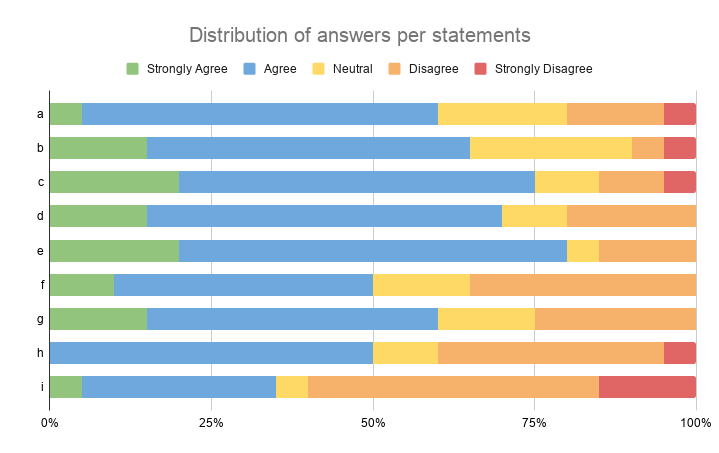
\includegraphics[width=\columnwidth]{StatementAnswers}
  \Description{Chart representing the distribution of answers per statement.}
  \caption[StatementResults]{Chart representing the distribution of answers per statement.}
  \label{fig:statementresult}
  \centering
\end{figure}

The results show that although more than half of the respondent (60\%) find technical debt to be a problem in their project, a majority (65\%) agree that technical debt is necessary in order to deliver.
Further, most respondents (75\%) consider their current level of debt acceptable.
This indicates that developers are facing the need to balance the problems caused by technical debt with the need to deliver in time and that this requires accepting a certain level of technical debt.

A greater part of the respondent indicate that they have a clear overview of both the amount of technical debt (70\%) and where the debt is located in the project (80\%).
However, only half of the respondents work in a project where technical debt is actively managed (50\%) or with a clear strategy for technical debt management (50\%), and a majority (60\%) does not experience that everyone in their team are aware of the technical debt strategy.
This points to a problem with an absence of awareness and communication about technical debt in many software development projects.

The second part of the survey included a collection of open ended questions about the respondents experience with technical debt in their daily work.
When asked how technical debt impacts their daily work the most common theme was that it leads to a slow down in the development process, results in longer time to deliver and limits the ability to add new features.
One respondent writes:
\begin{quote}
  "[It] takes longer time to deliver new features, onboard new team members, limits what solutions we can choose for problems." (respondent 17)
\end{quote}

Next, the respondents were asked to describe how they currently manage technical debt.
The most common answer was that they do it little by little as they stumbled upon it.
The "boy scout principle" was mentioned multiple times by different respondents.
One respondent explains:
\begin{quote}
  "Boy scout principle. Leave the code a little better than you found it." (respondent 11)
\end{quote}
Another aspect mentioned by multiple respondents is the difficulty managing a balance between paying off technical debt and adding new features as one respondent describes in the following statement: 
\begin{quote}
  "We write stories for it and add them to the backlog. Each sprint we include some such stories - but it's a bit of a tug of war with the business who wants more features instead." (respondent 16)
\end{quote}

When asked about what tools or processes the respondents currently are using to manage technical debt most of the respondents did not use any special tool but rather relied on their existing workflow for bug and feature tracking, code reviews and sprint meetings.

Lastly, the respondents were asked what features they would want in a tool designed to help manage technical debt.
Among the many different answers there were a few recurring suggestions for features or important aspects of such a tool.
Multiple respondents requested a way of understanding the balance between the cost of fixing instances of debt and the potential benefit gained by paying off the debt. An example is the following answer:
\begin{quote}
  "Wow, good question. Not sure, but I guess it'd important for me to somehow be able to see how 'expensive' a certain tech debt payoff project would be together with it's potential reward. This would make prioritization between different tech debt payoff projects better." (respondent 18)
\end{quote}
Another respondent describes a platform where you can document areas in the code where technical debt is present and keep track of the technical debt in the project:
\begin{quote}
  "A tool that could help us document part of the code we think as technical dept. A platform that we could have conversation about things and keep track of ideas how to solve things." (respondent 19)
\end{quote}
The idea of a tool to help a team schedule and prioritize technical debt also surface multiple times among the answers. One respondent writes:
\begin{quote}
  "Maybe a 'queue' of topics we have decided is tech debt and for how long they have not been addressed. Otherwise, a solution for the current standards and ways of working with notifications for 'now you have not reviewed this in X months'. Making a tool which proactively helps you schedule tech debt fixing which is open and transparent to both managers and developers." (respondent 15)
\end{quote} 